\documentclass{elsarticle}
\usepackage[utf8]{inputenc}
\usepackage[spanish,mexico]{babel}

\usepackage{hyperref}
% \usepackage{lineno,hyperref}
% \modulolinenumbers[5]

% \journal{Journal of \LaTeX\ Templates}

% \usepackage{natbib}

%%%%%%%%%%%%%%%%%%%%%%%
%% Elsevier bibliography styles
%%%%%%%%%%%%%%%%%%%%%%%
%% To change the style, put a % in front of the second line of the current style and
%% remove the % from the second line of the style you would like to use.
%%%%%%%%%%%%%%%%%%%%%%%

% Numbered
% \bibliographystyle{model1-num-names}

%% Numbered without titles
% \bibliographystyle{model1a-num-names}

%% Harvard
% \bibliographystyle{model2-names}\biboptions{authoryear}

%% Vancouver numbered
% \usepackage{numcompress}\bibliographystyle{model3-num-names}

%% Vancouver name/year
% \usepackage{numcompress}\bibliographystyle{model4-names}\biboptions{authoryear}

%% APA style
% \bibliographystyle{model5-names}\biboptions{authoryear}

%% AMA style
% \usepackage{numcompress}\bibliographystyle{model6-num-names}

%% `Elsevier LaTeX' style, distributed in TeX Live 2019
\bibliographystyle{elsarticle-num}
% \usepackage{numcompress}\bibliographystyle{elsarticle-num-names}
% \bibliographystyle{elsarticle-harv}\biboptions{authoryear}
%%%%%%%%%%%%%%%%%%%%%%%

\begin{document}

\begin{frontmatter}

\title{Seleccionar modelos de pronóstico para series de tiempo de contaminatnes de PM10 por criterio de Akaike y bayesiano\tnoteref{mytitlenote}}
\tnotetext[mytitlenote]{Fully documented templates are available in the elsarticle package on \href{http://www.ctan.org/tex-archive/macros/latex/contrib/elsarticle}{CTAN}.}

%% Group authors per affiliation:
\author{Alberto Benavides}
\address{Nuevo León, México}
% \fntext[myfootnote]{Since 1880.}

%% or include affiliations in footnotes:
% \author[mymainaddress,mysecondaryaddress]{Elsevier Inc}
% \ead[url]{www.elsevier.com}

% \author[mysecondaryaddress]{Global Customer Service\corref{mycorrespondingauthor}}
% \cortext[mycorrespondingauthor]{Corresponding author}
% \ead{support@elsevier.com}

% \address[mymainaddress]{1600 John F Kennedy Boulevard, Philadelphia}
% \address[mysecondaryaddress]{360 Park Avenue South, New York}

\begin{abstract}
Selecting time series by selection criteria models
\end{abstract}

\begin{keyword}
series de tiempo \sep AM \sep MA \sep ARMA \sep modelos de selección de criterios \sep Akaike \sep Bayes \sep AIC \sep BIC \sep PM10 \sep Monterrey
% \MSC[2010] 00-01\sep  99-00
\end{keyword}

\end{frontmatter}

% \linenumbers

\section{Introduction}

La capacidad de pronosticar acertadamente es una de las habilidades más valoradas en muchos de los ámbitos humanos que incluso aparece elogiado desde narraciones bíblicas y otras provenientes del periodo griego clásico \cite{Hyndman2018}. La certeza de estos pronósticos ha sido relevante en la prevención de desastres naturales \cite{Cheng2007}, el tratamiento preventido de determinadas enfermedades (principalmente cáncer \cite{Earnest2019, Kumar2014}) o la elección de estrategias ventajosas en operaciones bursátiles \cite{BabuASReddy2015, Xiao2014}. 

En los modelos de pronóstico es común utilizar estrategias intuitivas para elegir los parámetros con los que se harán las predicciones, sin embargo estas aproximaciones pueden considerarse poco formales como lo fueron las artes adivinatorias o proféticas representadas popularmente por Nostradamus \cite{Popkin1984}. 

En este artículo se pretenden utilizar criterios robustos para realizar la selección de parámetros en el pronóstico de contaminantes en el Área Metropolitana de Nuevo León, México (AMM). Para ello, se abordan en la sección \ref{mt} los fundamentos relacionados a las series de tiempo, sus características, modelos de pronóstico y los criterios con los que hará la selección de sus parámetros. Posteriormente, en la sección \ref{datos} se describen los datos, su origen, manipulación y preprocesamiento. Luego, se muestra en la sección \ref{metodologia} la metodología a la que se sometieron y los resultados obtenidos para, en la sección \ref{conclusiones}, mostrar las conclusiones obtenidas.

\section{Marco teórico}
\label{mt}

Las series de tiempo son conjuntos de observaciones tomadas a lo largo del tiempo sobre algún evento, formalmente definidas \cite{Wei2019} a partir del concepto de una familia de variables aleatorias $Z(\omega, t)$, con un espacio muestral $\omega$ y un conjunto de índices temporales $t$, en las que para una determinada $t$, $Z(\omega, t)$ es una variable aleatoria, y para una $\omega$ dada, $Z(\omega, t)$ es una \textbf{serie de tiempo} que, por comodidad, se denomina $Z_t$.

De estas series de tiempo se puede calcular su media
\begin{equation}
\mu_t = E(Z_t),
\end{equation}
y varianza 
\begin{equation}
\sigma^2_t = E(Z_t - \mu_t)^2;
\end{equation}
a partir de estas, la covarianza entre dos tiempos $t_1, t_2$
\begin{equation}
\gamma(t_1, t_2) = E(Z_{t_{1}} - \mu_{t_{1}}) E(Z_{t_{2}} - \mu_{t_{2}}),
\end{equation}
y la correlación también entre dos tiempos $t_1, t_2$
\begin{equation}
    \rho (t_1, t_2) = \frac{\gamma (t_1, t_2)}{\sigma_{t_{1}} \sigma_{t_{2}}}.
\end{equation}

Esto permite definir la \textbf{función de autocorrelación} (ACF) $\rho_k$ como la correlación que tiene una serie consigo misma en los tiempos $t_1 = 0, t_2 = k$, es decir
\begin{equation}
    \rho_k = \frac{\gamma_k}{\gamma_0}
\end{equation}

Ahora se introduce el concepto de \textbf{regresión lineal} entendida como la relación lineal entre la varialbe dependiente $X_i$ y la variable independiente $Y_i$ para $i = [1, \ldots, n]$, tal que
\begin{equation}
    Y_i = \beta_0 + \beta_1 X_i + \epsilon_i.
\end{equation}
Aquí, $\beta_0 + \beta_1 X_i$ son la función lineal que mejor se ajusta a $X_i$ con base en el menor de los errores cuadrados, mientras que $\epsilon_i$ es la distancia entre dicha recta y el valor de $Y_i$ para determinada $i$. Cuando se tienen $p$ variables dependientes $X_{ij}, j = [1, \ldots, p]$, la regresión lineal se escribe
\begin{equation}
\label{pacf}
    Y_i = \beta_0 + \beta_1 X_{i1} + \beta_2 X_{i2} + \ldots + \beta_p X_{ip} + \epsilon_i.
\end{equation}

Con esto, la \textbf{función de autocorrelación parcial} (PACF) para un retraso de $k$ unidades, queda definida a partir de la ecuación \ref{pacf} como
\begin{equation}
    Z_t = \beta_1 Z_{t-1} + \beta_2 Z_{t-2} + \ldots + \beta_k Z_{t-k} + \epsilon_t,
\end{equation}
siendo el coeficiente $\beta_k$ el que define la interacción del retraso $k$ en la serie de tiempo $Z_t$.

Ahora bien, un \textbf{modelo autorregresivo} (AR) es uno de los modelos utilizados para el pronóstico de series de tiempo. Este modelo se basa en la idea de que una serie de tiempo $Z_t$ puede ser pronosticada $Y_t$ a partir de la información proporcionada por las regresiones de momentos pasados de dicha serie de tiempo. A saber:
\begin{equation}
    Y_t = c + \phi_1 Y_{t-1} + \phi_2 Y_{t-2} + \ldots +  + \phi_p Y_{t-p} + \epsilon_t
\end{equation}
es el modelo autorregresivo de orden $p$, abreviado AR($p$). En este tipo de modelos, es una práctica común utilizar los valores significativos de la PACF de una serie de tiempo como los valores $p$ para obtener pronósticos.

Otro modelo utilizado para pronóstico es el \textbf{modelo de media móvil} en que en lugar de utilizar valores pasados de $Z_t$ para realizar el pronóstico, como en los AR, se usan los errores de pronóstico $\epsilon_t$ de las predicciones con diferentes retrasos y coeficientes $\theta$, por lo que
\begin{equation}
    Y_{t} = \epsilon_t + \theta_{1} \epsilon_{t-1} + \theta_{2}\epsilon_{t-2} + \ldots + \theta_{q}\epsilon_{t-q}.
\end{equation}

Estos dos modelos se combinan para formar el \textbf{modelo autorregresivo de media móvil} (ARMA) que tiene la forma
\begin{equation}
    Y_t = c + \phi_1 Y_{t-1} + \phi_2 Y_{t-2} + \ldots + \phi_p Y_{t-p} + \epsilon_t + \theta_{1} \epsilon_{t-1} + \theta_{2}\epsilon_{t-2} + \ldots + \theta_{q}\epsilon_{t-q},
\end{equation}
denominado ARMA($p$, $q$).

También, una serie de tiempo se puede entender a partir de su descomposición en la \textit{tendencia} $T_t$, los \textit{residuales} $R_t$ y la \textbf{estacionalidad} $S_t$ \cite{Brockwell2002}. La tendencia es equivalente a $\beta_0$ y los residuales a los $\epsilon_t$, mientras que la estacionalidad explica los patrones o ciclos que se hallan en las serie. Estas componentes pueden encontrarse sumadas
\begin{equation}
    Z_t = T_t + R_t + S_t
\end{equation}
o bien, multiplicadas:
\begin{equation}
    Z_t = T_t \times R_t \times S_t.
\end{equation}

Los modelos de pronóstico basados en el AR y MA son eficientes cuando se parte de una serie de tiempo \textbf{estacionaria}, esto es, aquella que tiene una media $\mu_t$ y varianza $\sigma^2_t$ constantes y no es estacional. Para determinar si una serie de tiempo es estacionaria, se cuenta con las pruebas de hipótesis de Dickey-Fuller aumentada (ADF) y la de Kwiatkowski-Phillips-Schmidt-Shinn (KPSS). 

La hipótesis nula de la prueba ADF es que la serie es no estacionaria con un valor $p = 0.05$. Cuando no se puede rechazar la hipótesis nula, es posible hacer una diferenciación $Z'_t$ de la serie de tiempo $Z_t$ mediante
\begin{equation}
\label{diferenciacion}
    Z'_t = Z_t - Z_{t - d}
\end{equation}
donde $d$ es el retraso dado. Al realizar este proceso, el modelo ARMA se llama ARIMA, donde la I viene de \textit{integrated} en inglés, que puede traducirse como diferenciada en este contexto. Se dice que se aplica un modelo ARIMA($p, d, q$) a partir de un modelo AR($p$), MA($q$) con una serie de tiempo diferenciada $d$ unidades.

A partir de la ACF, PACF de una serie de tiempo se pueden elegir las variables $p, f$ de un modelo ARMA o ARIMA a partir de los valores estadísticamente significativos de dichas series. Las combinaciones de estos valores pueden ser variadas e incluir más o menos parámetros en los modelos o más o menos exactitud respecto a la serie que se desea pronosticar, por lo que se utilizan algunos criterios para determinar cuáles son las mejores combinaciones de parámetros para este tipo de pronósticos. Los dos modelos más usados son el Akaike (AIC) y el bayesiano (BIC).

El criterio de información de Akaike se describe como
\begin{equation}
\mbox{AIC} = -2 \log{L} + 2 (p + q + d + 1),
\end{equation}
donde $L$ es la similitud (definida en la ecuación 7.7.2 de \cite{Hyndman2018}) entre la series de tiempo $Z_t$ y el modelo $Y_t$. Por último, el criterio de información bayesiano \cite{Albert2007} en series de tiempo depende del AIC, pero también toma en cuenta el número de muestras $n$ en el modelo, así que se puede escribir
\begin{equation}
    \mbox{BIC} = -2 \log(L) + \ln(n) \cdot (p + q + d + 1).
\end{equation}
Para estos criterios, es preferible un valor pequeño respecto a otro mayor porque esto implica el uso de menos parámetros $(p + q + d + 1)$ y una mayor semejanza $2\log{L}$ entre serie de tiempo y función pronosticada.

\section{Datos}
\label{datos}

La serie de tiempo que se desea pronosticar proviene de los registros de calidad de aire obtenidos del Sistema Integral de Monitoreo Ambiental de Nuevo León (México) \cite{aireNL} que cuenta con trece estaciones de monitoreo ambiental (cuya ubicación se muestra en la figura \ref{estaciones_amm}, p. \pageref{estaciones_amm}) que registan fecha y hora, estación meteorológica, presión atmosférica, precipitaciones, humedad, radiación solar, temperatura, velocidad, dirección del viento y los contaminantes CO, NO, NO$_2$, O$_3$, SO$_2$, PM10, PM2.5. Algunas de estas estaciones registran datos desde 1993, y sólo coinciden su operación a partir de 2017, como se muestra en la figura \ref{estaciones_rangos} (p. \pageref{estaciones_rangos}). 

\begin{figure}
\centering
	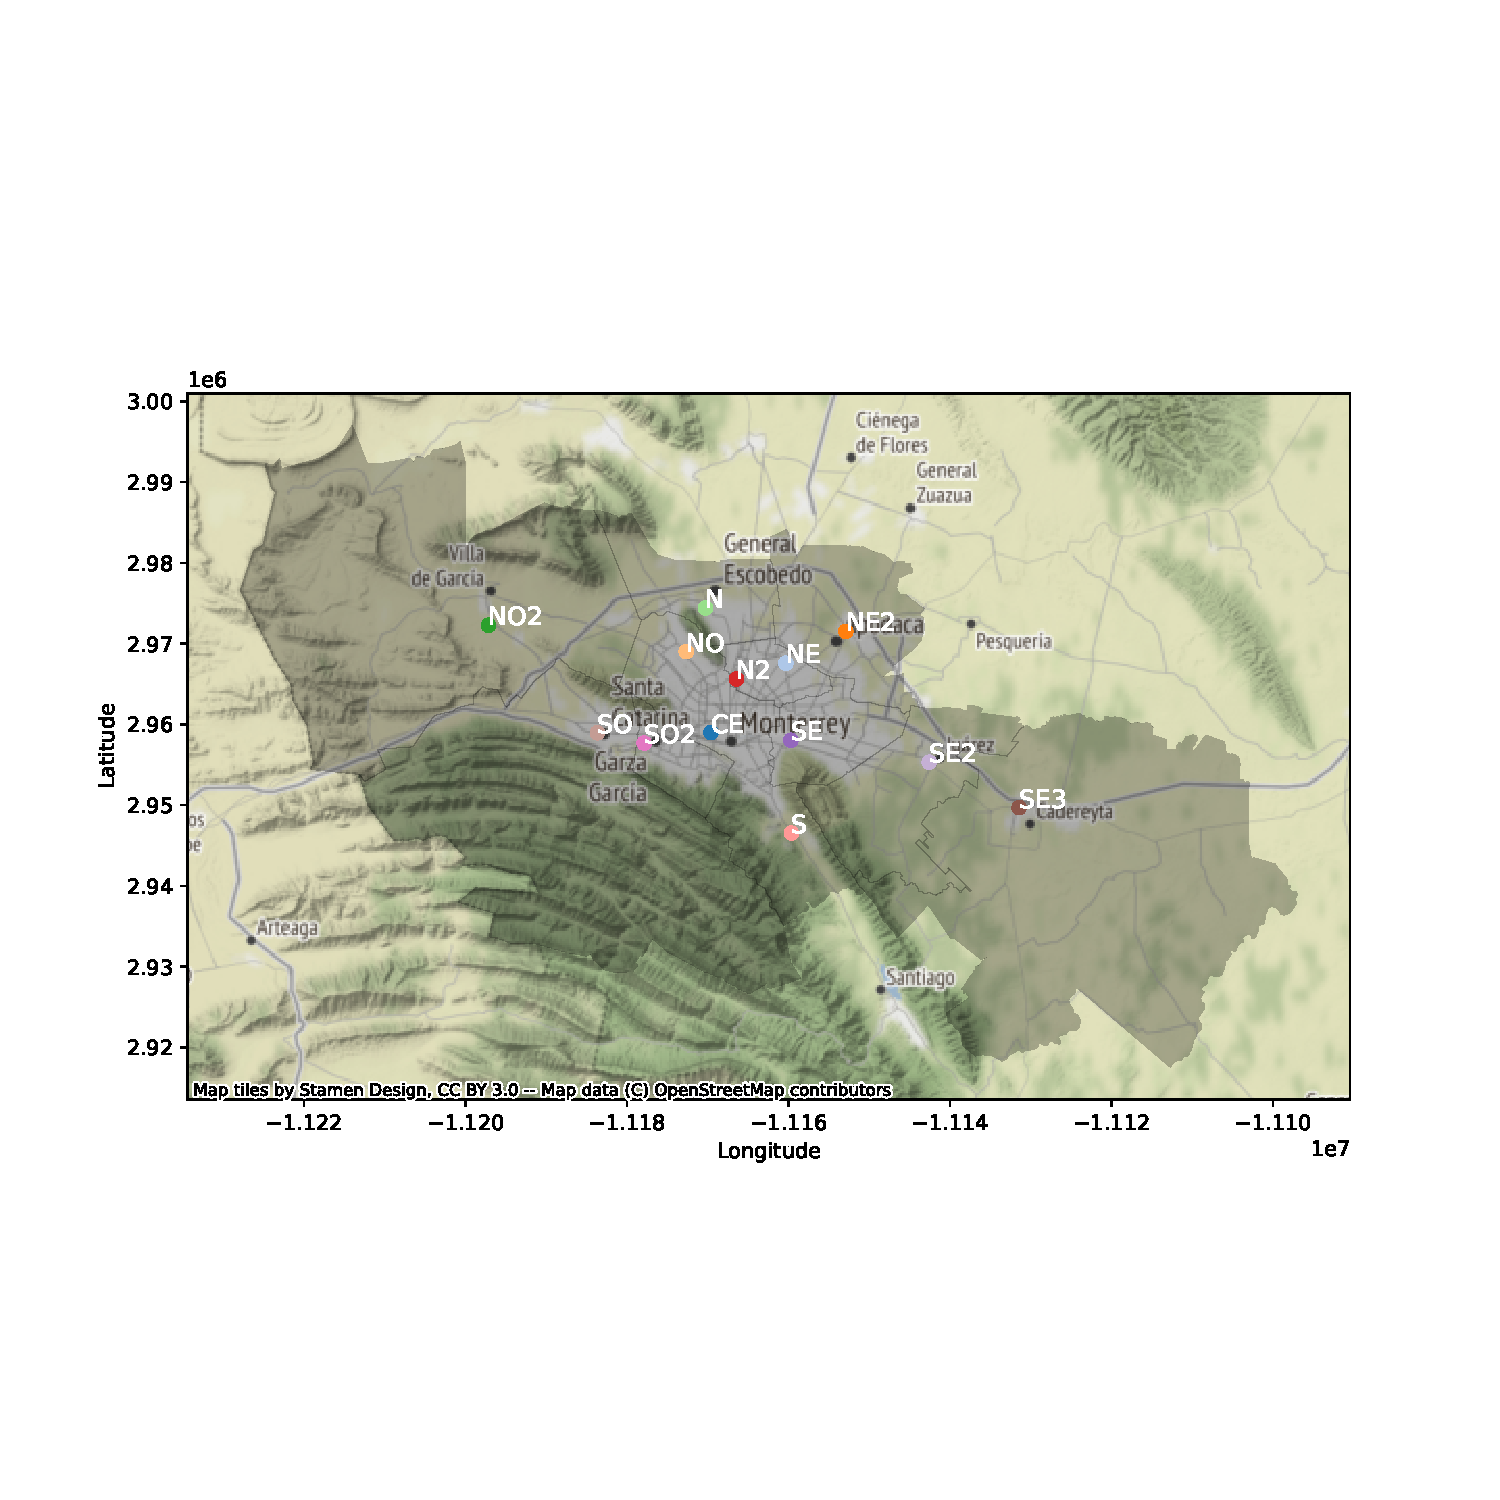
\includegraphics[width=1\textwidth]{estaciones_amm.pdf}
	\caption{Trece estaciones de monitoreo del Área Metropolitana de Monterrey (Nuevo León, México)}
	\label{estaciones_amm}
\end{figure}

\begin{figure}
\centering
	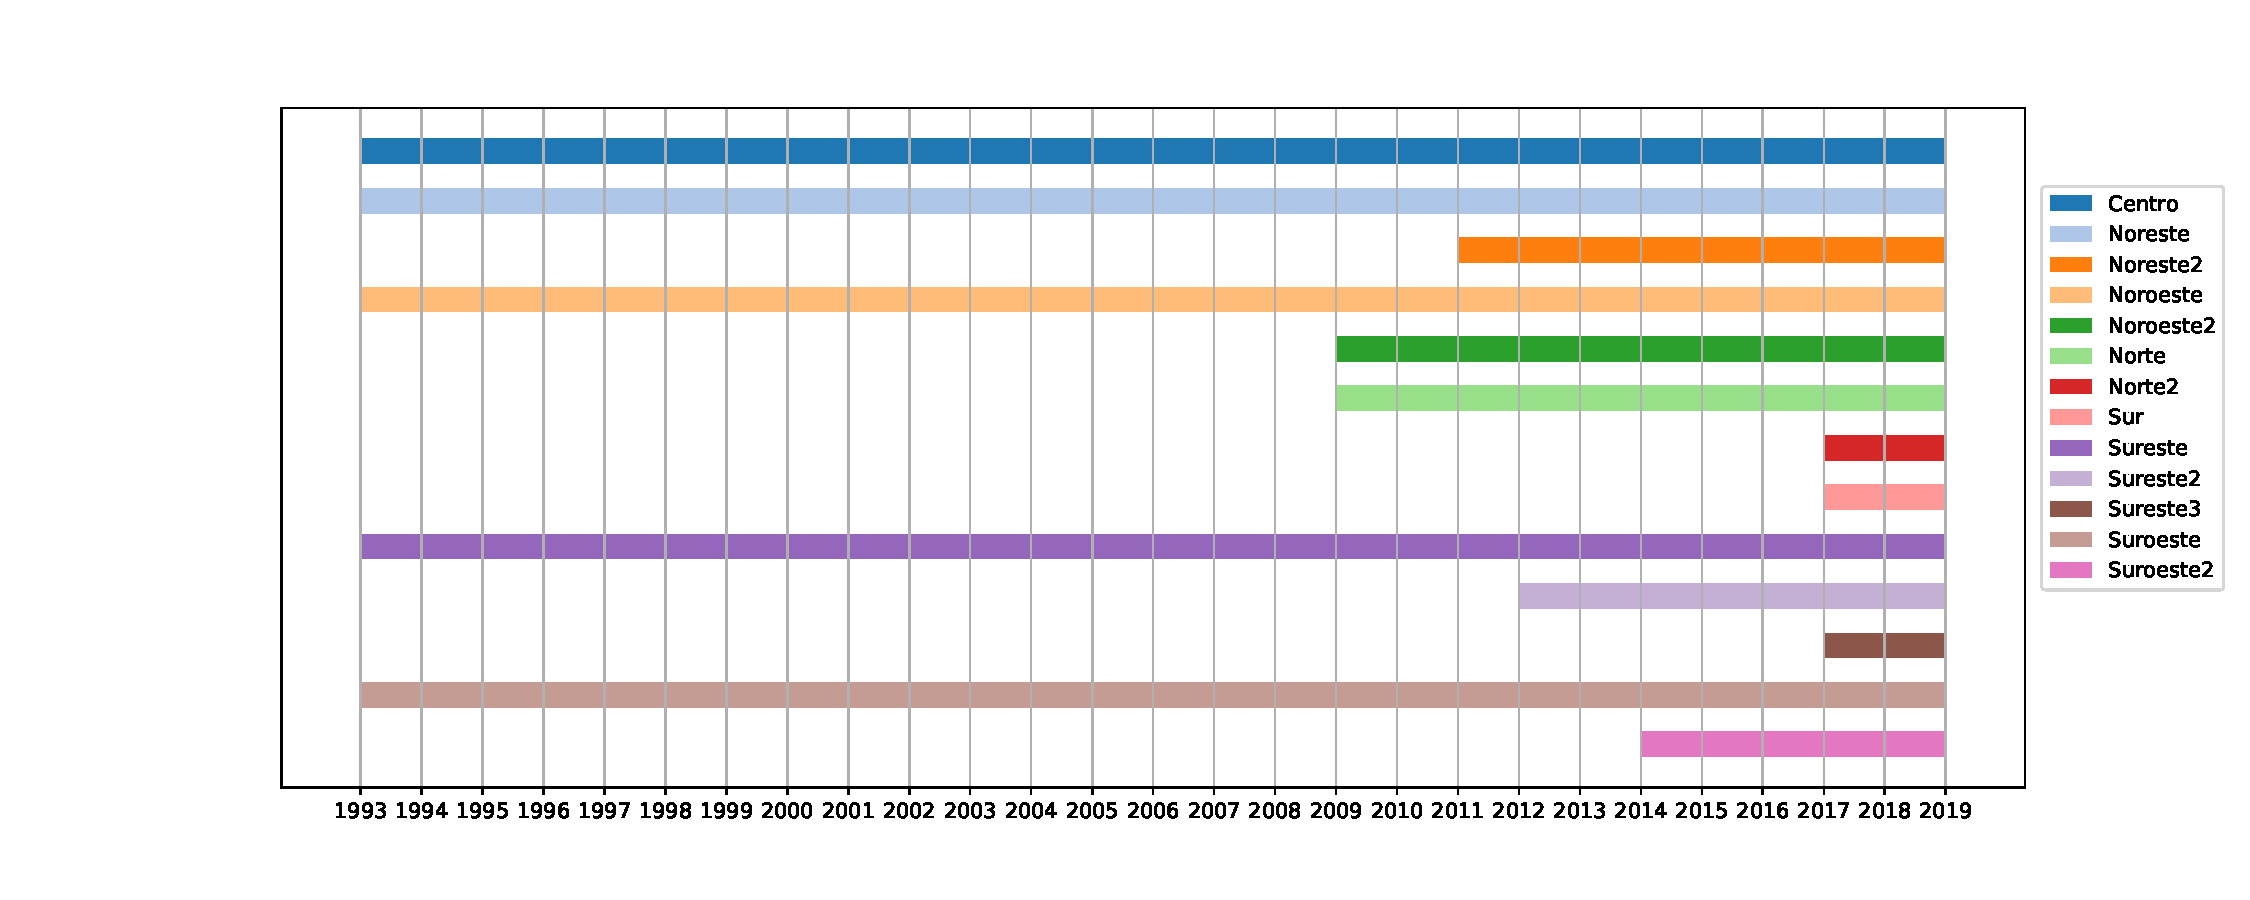
\includegraphics[width=1\textwidth]{estaciones_rangos.pdf}
	\caption{Barras de tiempo en que han estado activas las estaciones de monitoreo del AMM.}
	\label{estaciones_rangos}
\end{figure}

Se llaman contaminantes PM10 a los que tienen que ver con partículas suspendidas con tamaño menor o igual a $10 \mu$m. Las altas concentraciones de estos contaminantes están relacionadas con enfermedades respiratorias \cite{Pope1991} y muertes prematuras en población de riesgo \cite{Ito1996}. 

Su estudio resulta interesante porque porque la Secretaría de Gobernación de México publicó la norma Norma NOM-172-SEMARNAT-2019 \cite{semarnat} en la que determina las concentraciones en las que el contaminante PM10 se consideran malas, mismas que se hallan en el cuadro \ref{semarnat} (p. \pageref{semarnat}). Al extraer los datos de PM10 durante el 2017 en el AMM, se comprueba que al menos un $65\%$ de los registros tienen una calidad considerada mala por la Secretaría de Gobernación de México, lo cual puede constatarse en la figura \ref{ts_2017_pm10} (p. \pageref{ts_2017_pm10}).

\begin{table}
	\centering
	\caption{Índice de aire y salud para PM10.}
	\label{semarnat}
	\begin{tabular}{|l|l|r|}
	\hline
	\textbf{Calidad del aire}  & \textbf{Nivel de riesgo} & \textbf{12 horas ($\mu$g / m$^3$)} \\ 
	\hline
	Buena & Bajo & $[0, 50)$ \\
	Aceptable & Moderado & $[50, 75)$ \\
	Mala & Alto & $[75, 155)]$ \\
	Muy mala & Muy alto & $[155, 235)]$ \\
	Extremadamente mala & Extremadamente alto & $> 235$ \\
	\hline
	\end{tabular}
\end{table}

\begin{figure}
\centering
	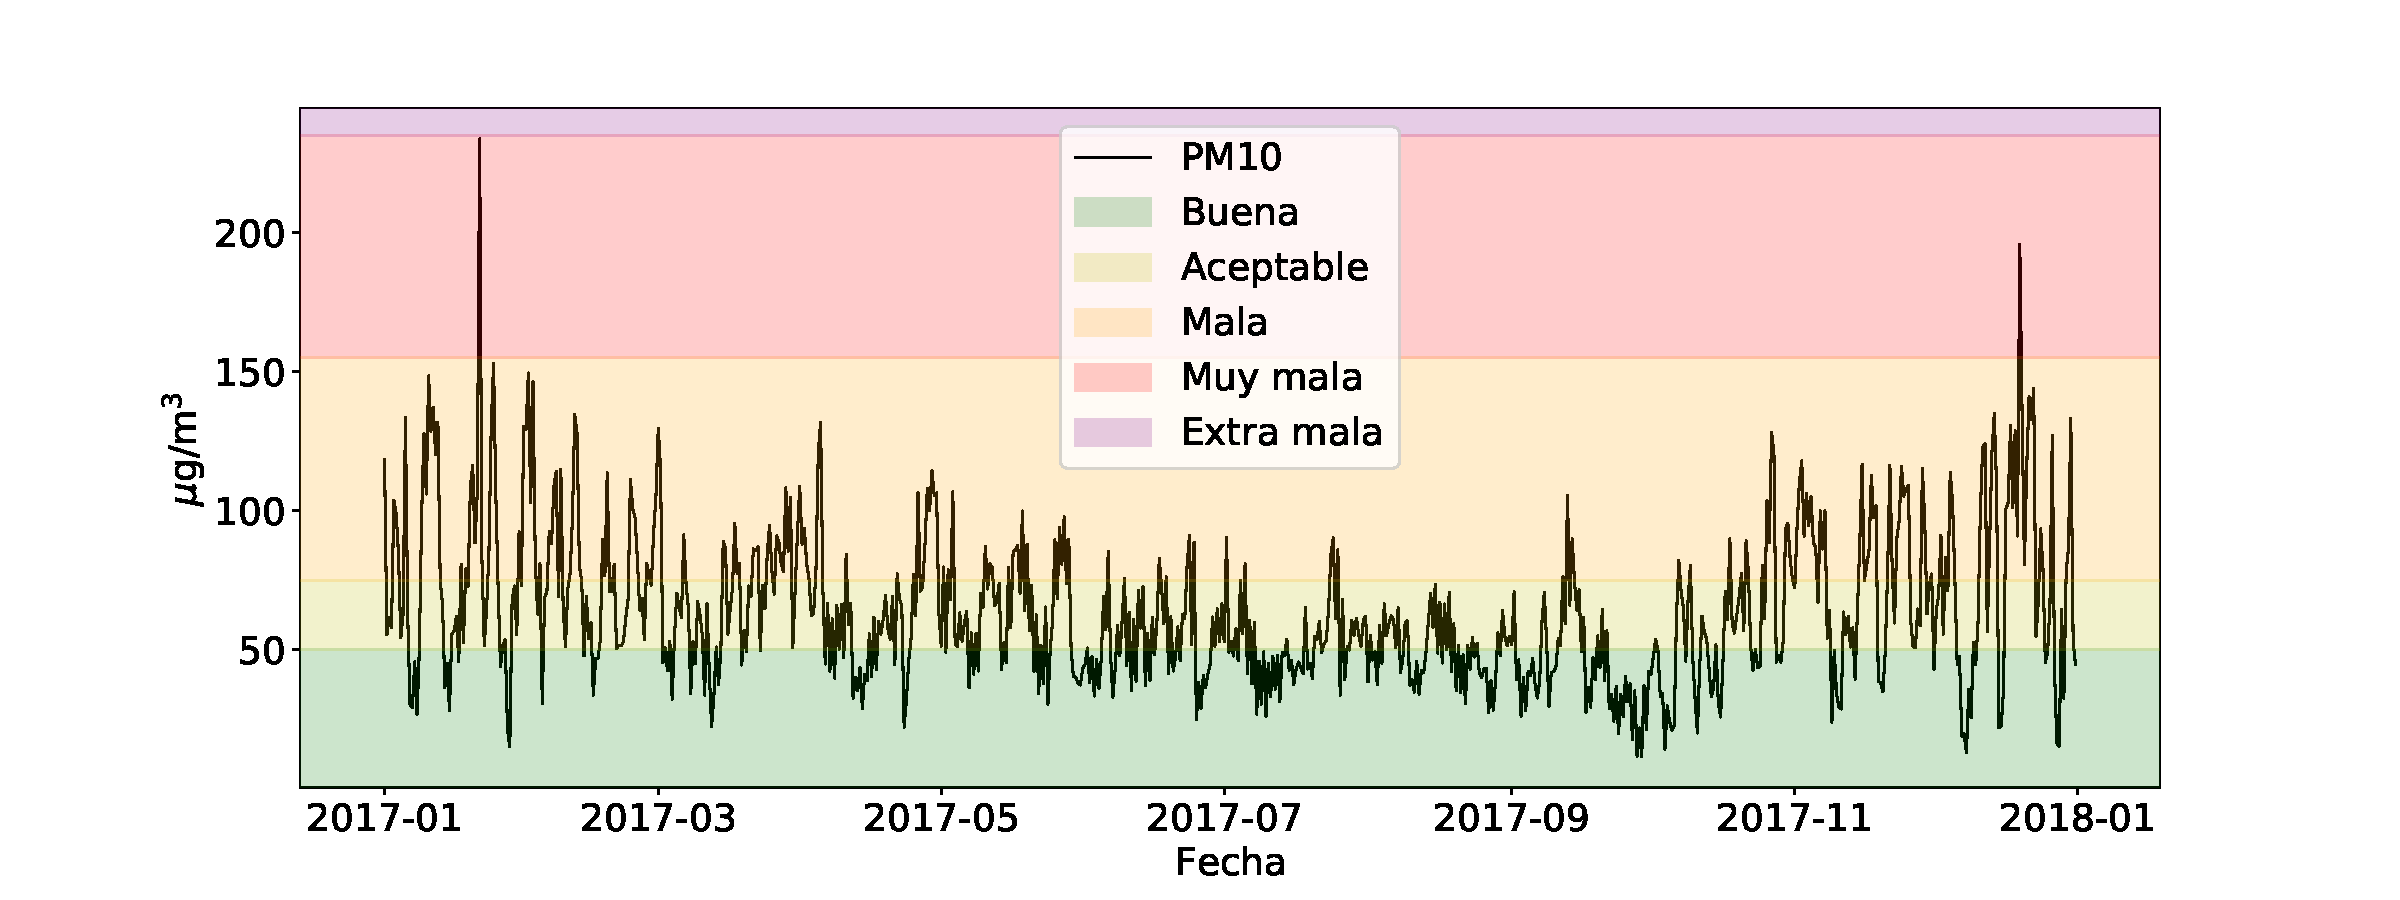
\includegraphics[width=1\textwidth]{ts_2017_pm10.pdf}
	\caption{Serie de tiempo de PM10, durante el año 2017 para el AMM.}
	\label{ts_2017_pm10}
\end{figure}

\section{Metodología y resultados}
\label{metodologia}
La serie de tiempo se descompuso en las componentes de tendencia, estacionalidad y residuales, como se muestra en la figura \ref{decompose_PM10_2017} (p. \pageref{decompose_PM10_2017}). En estas imágenes, se puede observar que la tendencia $\beta_0$ no se mantiene constante, por lo que se realiza la prueba de Dickey-Fuller aumentada y se obtiene un valor $p = 0.51$, por lo que no se puede rechazar la hipótesis de que la serie no es no estacionaria, de modo que se debe hacer una diferenciación de la misma aplicando la ecuación \ref{diferenciacion}. La serie tuvo que ser diferenciada dos veces, por lo que $d = 2$. La serie de tiempo original y la diferenciada con $d = 2$ están plasmadas en la figura \ref{df_PM10_diff2}.

\begin{figure}
\centering
	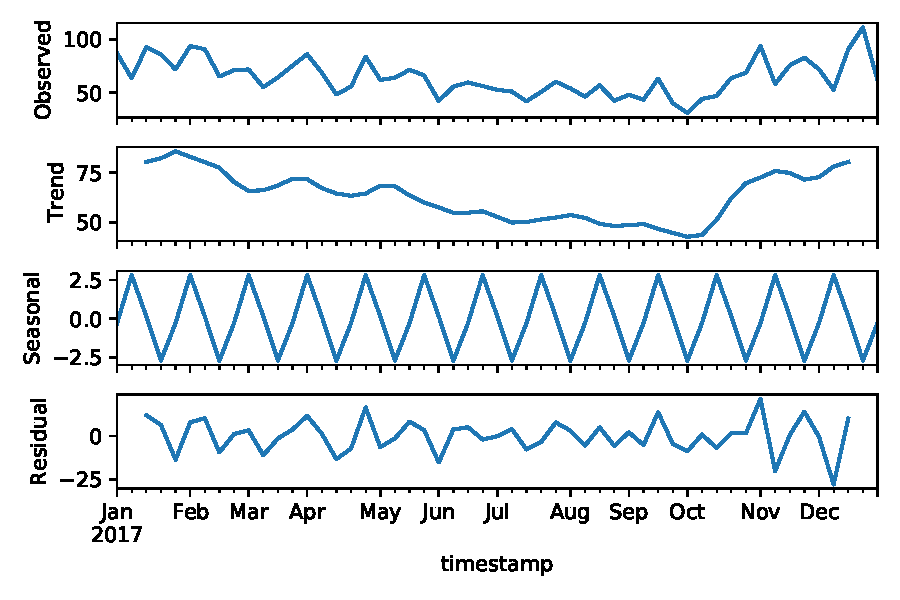
\includegraphics[width=1\textwidth]{decompose_PM10_2017.pdf}
	\caption{Serie de tiempo de PM10 de 2017 descompuesta en tendencia, estacionalidad y residuales.}
	\label{decompose_PM10_2017}
\end{figure}

\begin{figure}
\centering
	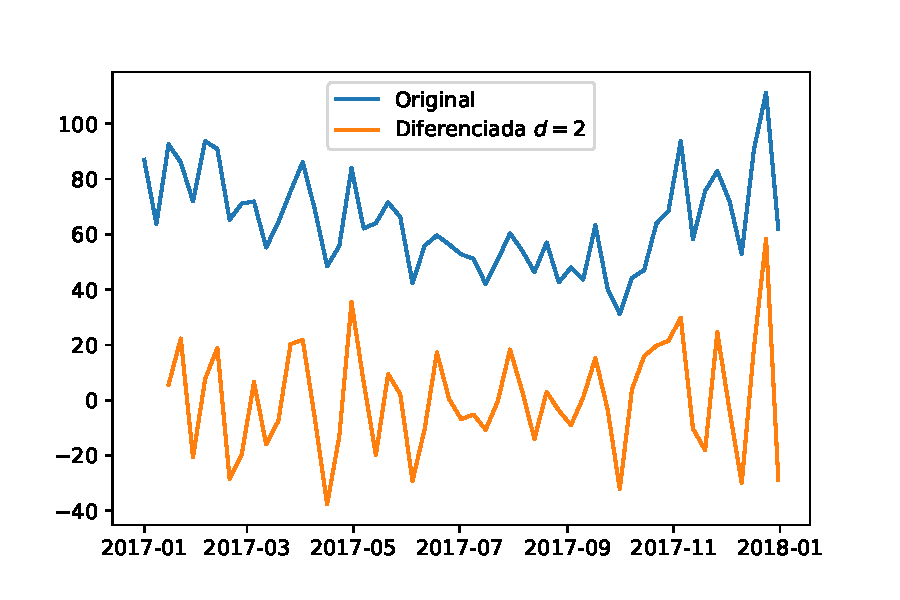
\includegraphics[width=1\textwidth]{df_PM10_diff2.pdf}
	\caption{Serie de tiempo de PM10 de 2017 (azul) y la diferenciada en $d = 2$ (naranja).}
	\label{df_PM10_diff2}
\end{figure}

También se obtuvieron sus ACF y PACF, incluidas en las figuras \ref{acf_PM10_2017_df2} y \ref{acf_PM10_2017_df2} (p. \pageref{pacf_PM10_2017_df2}). En este caso, no hay manera de seleccionar por ninguna de las funciones de correlación un buen conjunto de parámetros, por lo que se procederá a generar modelos ARIMA($p, 2, q$) con $p = [1, \ldots, 10], q = [1, \ldots, 10]$, de los que se calcula el AIC y BIC, además de la suma de ambos y luego se muestran los diez menores valores de AIC $+$ BIC y sus configuraciones de $p$ y $q$ en la tabla \ref{aicbic} (p. \pageref{aicbic}). En estos datos, se ve que la mejor combinación de valores es el modelo ARIMA($2, 2, 5$).

\begin{figure}
\centering
	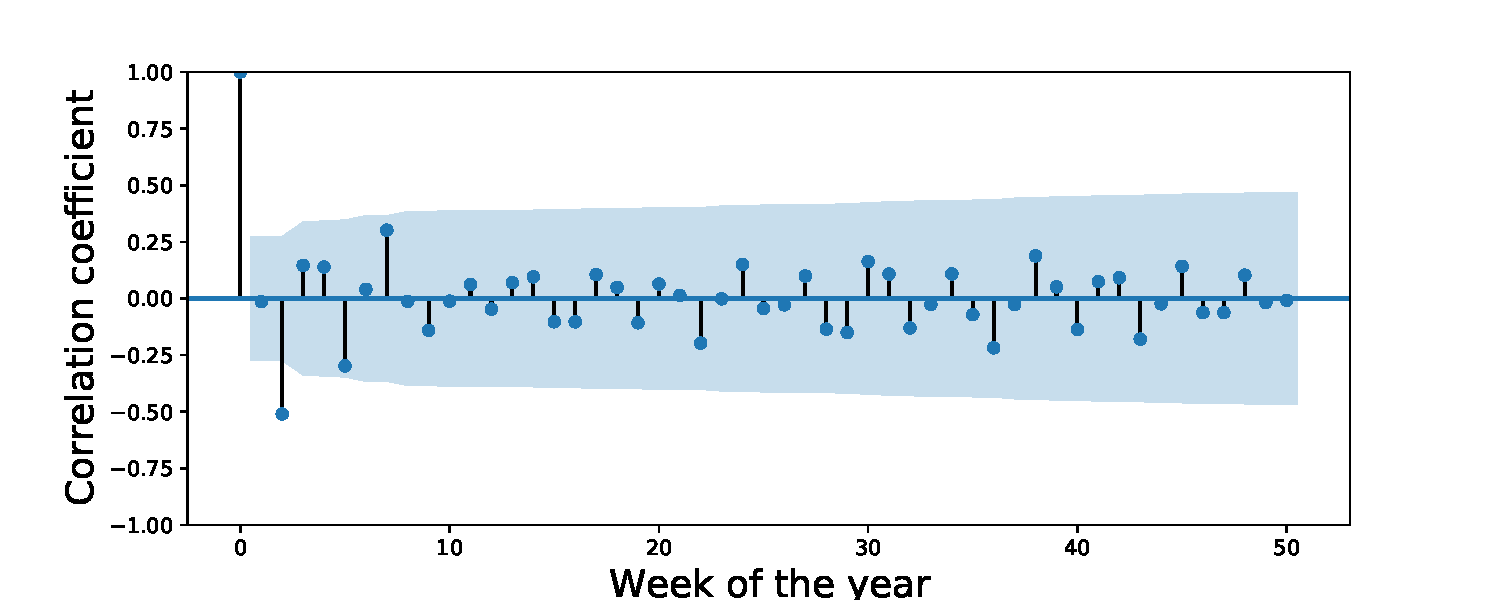
\includegraphics[width=1\textwidth]{acf_PM10_2017_df2.pdf}
	\caption{Coeficientes de autocorrelación para PM10 durante 2017 en el AMM.}
	\label{acf_PM10_2017_df2}
\end{figure}

\begin{figure}
\centering
	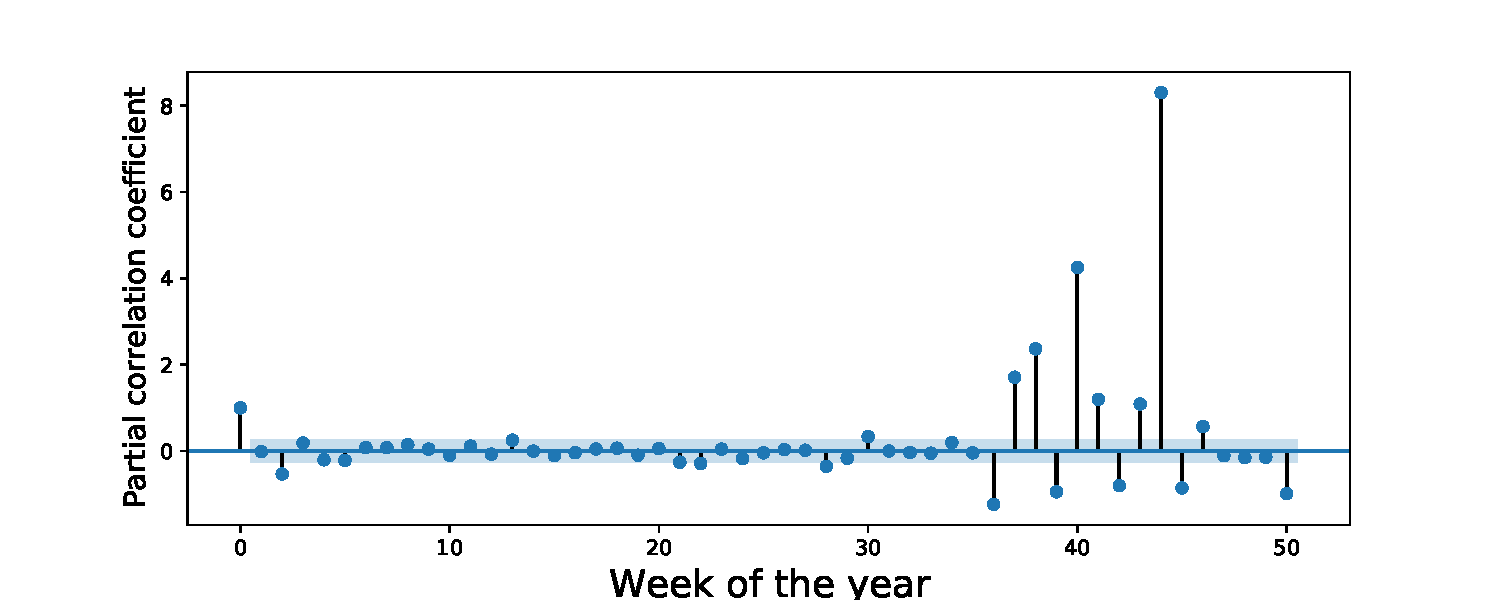
\includegraphics[width=1\textwidth]{pacf_PM10_2017_df2.pdf}
	\caption{Coeficientes de autocorrelación parciales para PM10 durante 2017 en el AMM.}
	\label{pacf_PM10_2017_df2}
\end{figure}

\begin{table}
	\centering
	\caption{Diez mejores combinaciones de $p$ y $q$ para ARIMA con base en la suma de AIC $+$ BIC.}
	\label{aicbic}
        \begin{tabular}{|c|c|c|c|c|}
        \hline
        $p$ &  $q$ &         AIC &         BIC &     AIC + BIC \\
        \hline
        2 &  5 &  422.78 &  439.80 &   862.58 \\
        5 &  2 &  424.32 &  441.35 &   865.66 \\
        4 &  3 &  424.36 &  441.38 &   865.74 \\
        2 &  3 &  427.56 &  440.80 &   868.36 \\
        1 &  4 &  427.60 &  440.84 &   868.45 \\
        6 &  6 &  421.36 &  447.85 &   869.21 \\
        5 &  6 &  423.18 &  447.77 &   870.95 \\
        2 &  4 &  428.02 &  443.16 &   871.18 \\
        6 &  1 &  430.17 &  447.20 &   877.37 \\
        5 &  1 &  431.18 &  446.32 &   877.50 \\
        \hline
        \end{tabular}
\end{table}

\section{Conclusiones}
\label{conclusiones}

Las dificultades que los modelos de pronóstico, como el ARIMA, presentan es que el tanteo de los parámetros del modelo de pronóstico pueden no conseguirse intuitiva ni directamente a partir de las ACF, PACF y diferenciación necesaria por prueba de estacionaridad. Los criterios de selección de modelos de Akaike y bayesiano resultan una herramienta estadística eficiente para solventar estas limitaciones. En general, sin embargo, es recomendable seguir la metodología descrita para tener una mejor información de la serie de tiempo que se desee pronosticar, pues desde la descomposición se tiene información relevante en la planeación de los modelos y estrategias a seguir en el pronóstico.

\bibliography{mybibfile}

\end{document}